\section{Results} \label{subm}
\subsection{COVID-19 Spike Protein Structure}
\hspace{5mm} To begin with, understanding the structure of COVID-19 is essential to comprehend how it affects humans. The virus has a unique structure that includes a spike protein called 6VXX (Structure of the SARS-CoV-2 spike glycoprotein). The spike protein, also known as the S protein, plays a crucial role in the virus's receptor recognition and cell membrane fusion process. This protein is made up of two subunits, S1 and S2. The S1 subunit contains a receptor-binding domain that specifically binds to the host receptor angiotensin-converting enzyme 2. On the other hand, the S2 subunit facilitates viral cell membrane fusion through the formation of a six-helical bundle via the two-heptad repeat domain. Recent research advancements have shed light on the development of antiviral drugs that target the S protein (Huang et al., 2020). Fig 1 shows the simulated protein structure of the S protein of COVID-19.

\vspace{5mm}

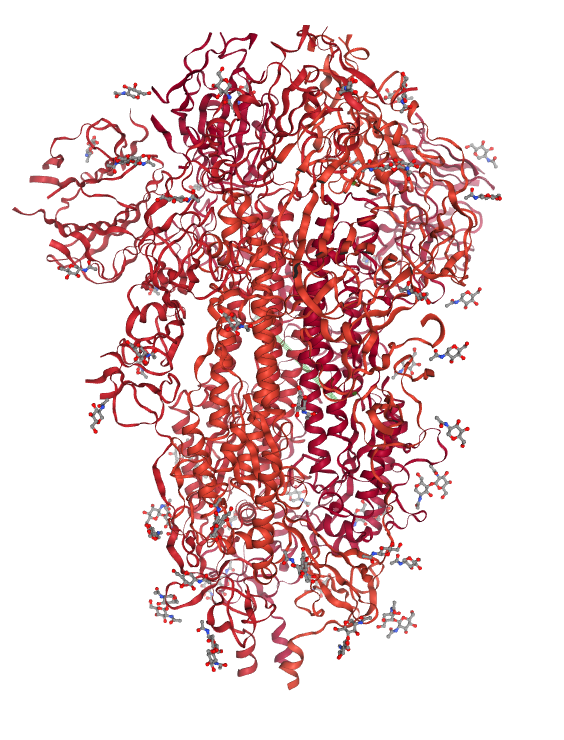
\includegraphics[width=6cm, height=6cm]{img/spike.png} 
\hspace{5mm}
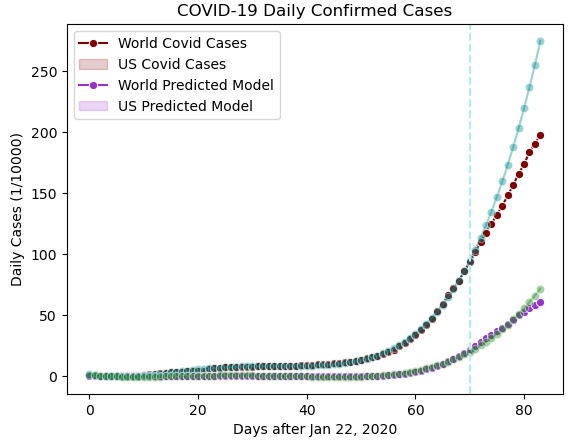
\includegraphics[width=8cm, height=6cm]{img/COVID19_confirmed.png}

Fig 1. 6VXX COVID-19 S protein \hspace{5mm}Fig 2. COVID-19 Confirmed Cases Prediction

\subsection{Statistical Analysis of COVID-19 Confirmed Cases}
\hspace{5mm} Figure 2 depicts the confirmed cases of COVID-19 provided by the WHO from January 22, 2020, to April 14, 2020. As the graph shows, the number of cases increases over time. It's important to note that this data was collected before the vaccine was developed and before many regulations were put in place.

\begin{center}
    \Large$\large y_j = \sum_{n=1}^N a_nt^n$; $j = 0,1,...,M$
\end{center}

The equation above shows the statistical power series model that I used to create Figure 2 after March 31, 2020. As shown, the prediction model is precise enough to estimate the future number of confirmed cases. However, it's important to note that this estimate is based on only three months of data and is not suitable for predicting the behavior of the infection in the long term. There are many unexpected factors that can influence infection rates, such as developments in vaccination and travel restrictions. While this model can provide an estimate of the number of COVID-19 patients, it's not suitable for describing the behavior of COVID-19.

\pagebreak
\subsection{Generalized Lokta-Volterra Model}
\hspace{5mm} As described in the background section, the generalized Lokta-Volterra (gLV) Model can simulate the ecological behaviors of many species. One well-known use of this model is to describe interactions within microbial communities (Venturelli1 et al., 2018). However, in the research conducted by Younes and Hasan (2020), the model was used to simulate the interactions between healthy and infected human populations. In their study, Younes and Hasan (2020) created a hypothetical country with a population of 100 people, consisting of 50 healthy individuals and 50 infected individuals. At the time of the study, no control measures were in place as there was no available data. In the optimal solution shown in Figure 03, no one travels or immigrates ($\alpha = 0$), resulting in a zero infection rate ($\beta = 0$). The recovery rate of 0.25 is based on the global average ($\gamma = 0.25$), while the birth and death rates are 0.01 and 0.001, respectively.

\vspace{5mm}
\hspace{-6mm}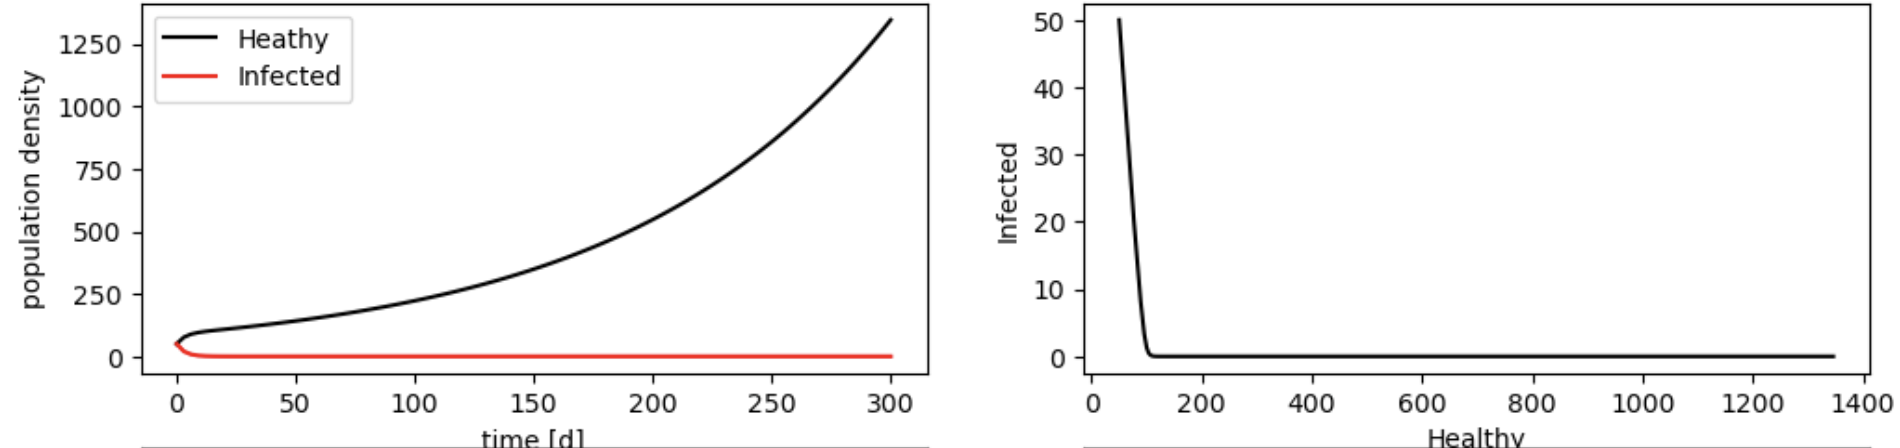
\includegraphics[width=16cm, height=5.2cm]{img/optimal_case.png}

\vspace{3mm}
\hspace{37mm} Figure 3. Optimal Case - No Immigration

\vspace{3mm}
Figure 3 shows that the number of infected people decreases in a short period of time, while the number of healthy individuals grows due to the birth rate. This could explain how the pandemic might have ended early if no one had been traveling.

\vspace{5mm}
\hspace{-6mm}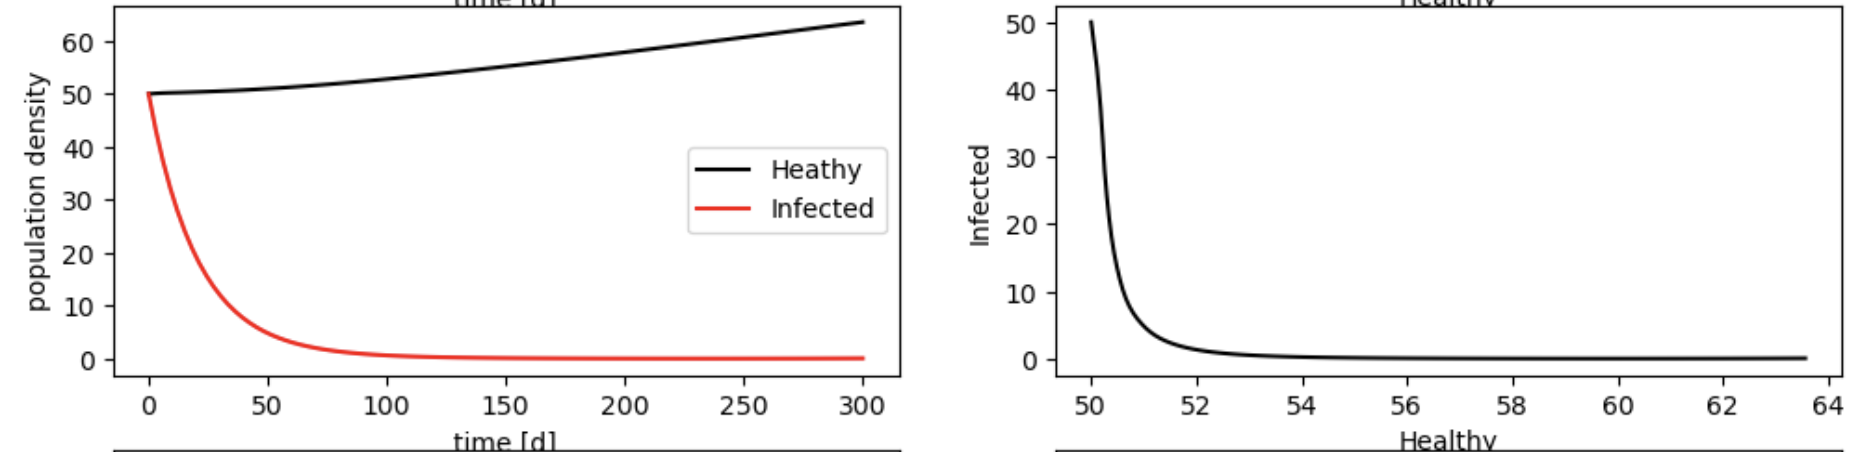
\includegraphics[width=16cm, height=5.2cm]{img/second_case_low_infection.png}

\vspace{5mm}
\hspace{37mm} Figure 4. Immigration 0.001 but Low Infection Rate
\vspace{5mm}

Figure 4 shows a graph of the immigration rate of 0.001 and an infection rate of 0.005. Although the decrease in the infected population is slower than in the optimal case (Figure 03), the infected population eventually reaches zero, and the pandemic comes to an end.


\hspace{-6mm}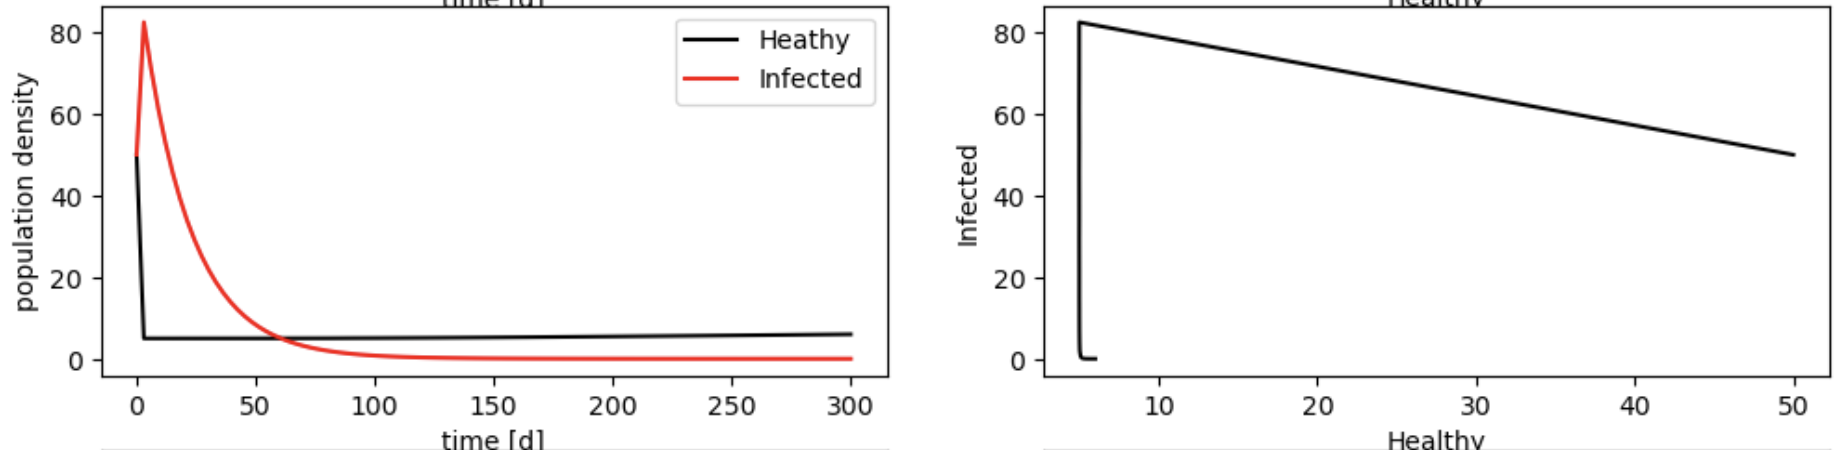
\includegraphics[width=16cm, height=5.2cm]{img/third_case_high_infection.png}

\vspace{3mm}
\hspace{30mm} Figure 5. Immigration 0.001 but a High Infection Rate

\vspace{3mm}

The conditions for Figure 05 are identical to those for Figure 04, except for the infection rate, which is 0.05 compared to 0.005 in Figure 04. Unlike in Figure 04, infected individuals in Figure 05 spread the disease to everyone in the healthy population, and within several days, no one in the country remains healthy. Due to the death rate of 0.05, the total population eventually reaches zero. Although people can recover from the disease, in the simulations, it is likely that they will become re-infected due to the high number of people who were previously infected.

\subsection{Generalized Lokta-Volterra Model with Controls}

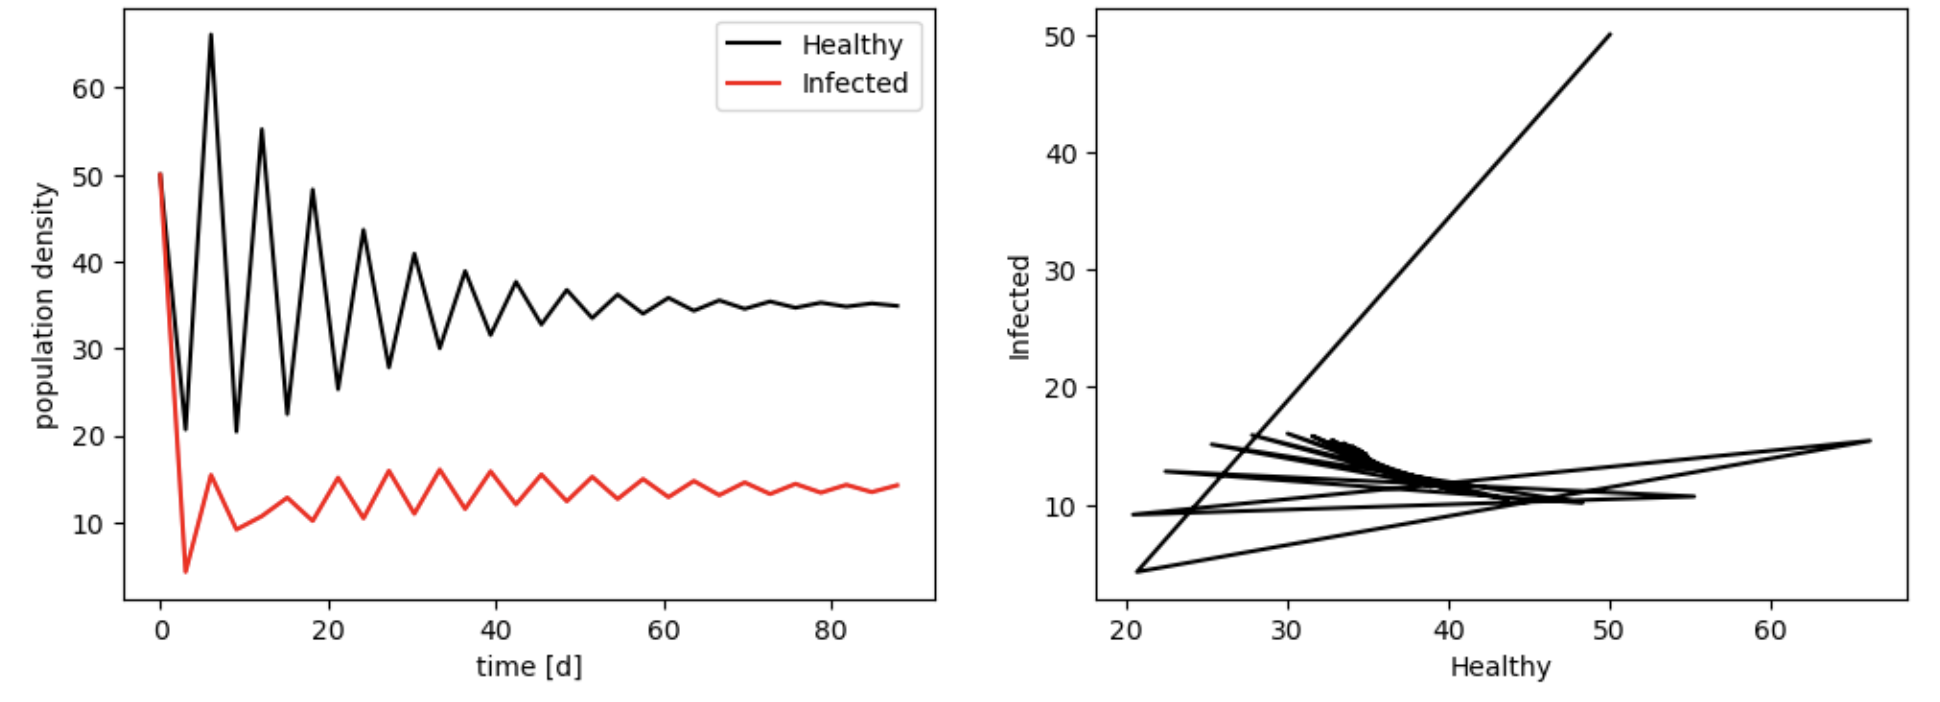
\includegraphics[width=16cm, height=5.2cm]{img/with_control.png}

\vspace{3mm}
\hspace{30mm} Figure 6. Vaccine, Treatments, and Five Controls

\vspace{3mm}

According to the CDC, 2 doses of monovalent mRNA COVID-19 vaccine were 36\% effective against COVID-19–associated hospitalization. Also, Sotrovimab, one of the COVID-19 treatments available, showed 79\% reduced chances of hospitalization. In this analysis, $\epsilon_H = 0.36, \epsilon_I = 0.79$ was used. for $u = [0.53, 0.11, 0.35, 0.41, 0.25]$, it represents border restriction, actively communicate with healthcare professionals, increase governmental support to vulnerable populations (41\%) and national lockdown (25\%) (Haug et.al., 2020).


Figure 6 demonstrates the interactions between healthy and infected populations in the presence of vaccines, treatments, and controls. The zig-zag shaped graph illustrates the behavior of the population with the implementation of controls. For instance, when the number of healthy individuals peaks, it decreases due to the infection, but it quickly recovers within a short time due to the implemented controls. Although the infection may continue to affect society over time, it stabilizes. Therefore, this analysis suggests that COVID-19 may not be eradicated, but the impacts on population numbers would be minimal. In other words, we will learn to coexist with COVID-19.